% =================================================================================================
% File:			registrazione_e_autenticazione.tex
% Description:	Definisce la sezione relativa ad un capitolo del documento
% Created:		2015-04-21
% Author:		Santacatterina Luca
% Email:		santacatterina.luca@mashup-unipd.it
% =================================================================================================
% Modification History:
% Version		Modifier Date		Change											Author
% 0.0.1 		2015-05-24 			inizio stesura sezione capitolo					Santacatterina Luca
% =================================================================================================
%

% CONTENUTO DEL CAPITOLO
\section{Autenticazione} % (fold)
\label{sec:autenticazione}
	In questa sezione saranno descritte le funzionalità di autenticazione\gloss{} fornite all'utente nella fase iniziale.

		\subsubsection{Autenticazione utente} % (fold)
		\label{sec:autenticazione_utente}
			Per effettuare l'autenticazione\gloss{} all'applicazione si devono inserire:
			\begin{itemize}
				\item Email;
				\item Password.
			\end{itemize}
			\begin{figure}[H]
				\centering
				\centerline{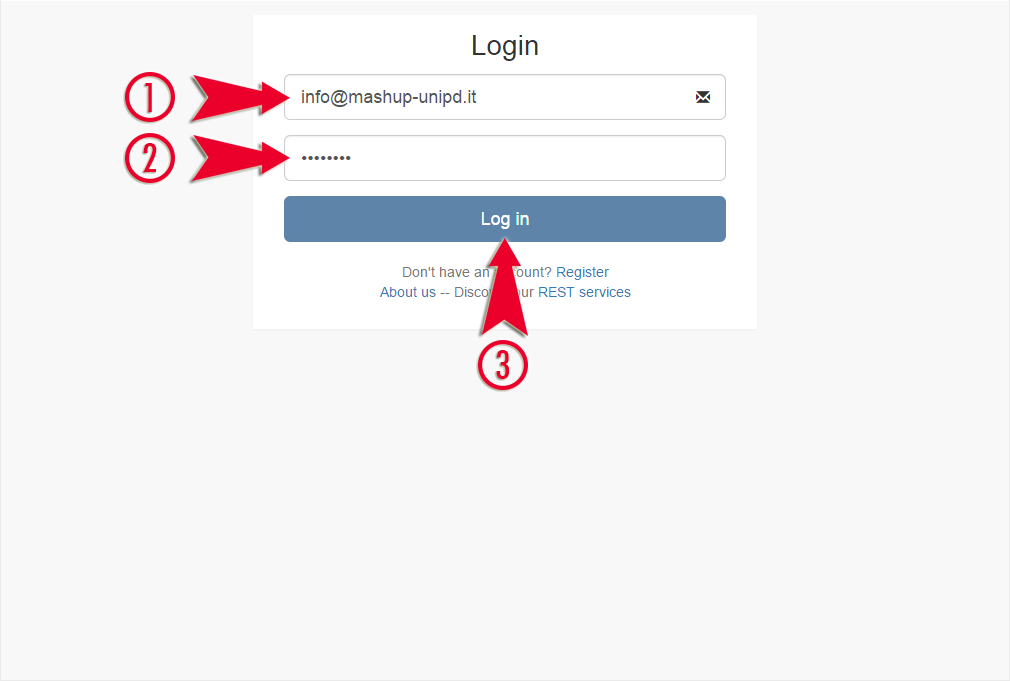
\includegraphics[width=14cm]{images/autenticazione_utente.png}}
				\caption{Autenticazione utente}
				\label{fig:registrazione_utente_accesso}
			\end{figure}
			Dopo aver inserito i dati di autenticazione (Figura \ref{fig:registrazione_utente_accesso}) sarà possibile premere il pulsante \textbf{Login}\gloss{} e quindi si verrà collegati alla dashboard\gloss{} dell'applicazione (Figura: \ref{fig:dashboard})
			\begin{figure}[H]
				\centering
				\centerline{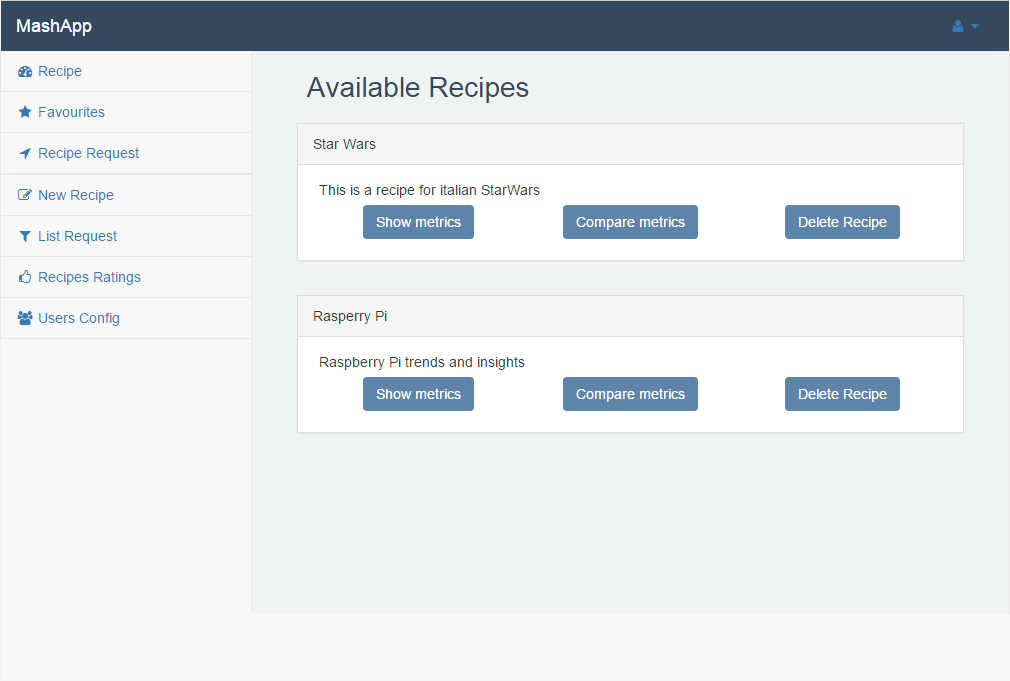
\includegraphics[width=19cm]{images/dashboard_amministratore.png}}
				\caption{Dashboard applicazione}
				\label{fig:dashboard}
			\end{figure}
		% section Autenticazione utente (end)


	% section Registrazione (end)

% section Registrazione e autenticazione (end)